\documentclass[dvipdfmx]{beamer}
\usetheme{metropolis}           % Use metropolis theme
\usepackage{float}
\usepackage[hang,small,bf]{caption}
\usepackage[subrefformat=parens]{subcaption}
\captionsetup{compatibility=false}
\usepackage{listings,jvlisting} %日本語のコメントアウトをする場合jvlisting(もしくはjlisting)が必要
%ここからソースコードの表示に関する設定
\lstset{
  basicstyle={\ttfamily},
  identifierstyle={\small},
  commentstyle={\smallitshape},
  keywordstyle={\small\bfseries},
  ndkeywordstyle={\small},
  stringstyle={\small\ttfamily},
  frame={tb},
  breaklines=true,
  columns=[l]{fullflexible},
  numbers=left,
  xrightmargin=0zw,
  xleftmargin=3zw,
  numberstyle={\scriptsize},
  stepnumber=1,
  numbersep=1zw,
  lineskip=-0.5ex
}

\title{Progress}
\date{\today}
\author{Mizuno Yasuaki}
%\institute{Centre for Modern Beamer Themes}
\begin{document}
  % 表紙の作成
  \maketitle
  
  \begin{frame}{ファミリー数削減}
    前回はファミリー数を百前後で学習を行ったが、ファミリー数を十に減らして、
    様々なニューラルネットワークのモデルを試す。ファミリー数を減らしたときのデータの構成を
    表\ref{tab:composition}に示す。
    \begin{table}
      \caption{削減データ(訓練データ)の構成\footnote{sum=5370, kind=10}}
      \label{tab:composition}
      \centering  
      \begin{tabular}{llll}
        \hline
        family & count & family & count \\
        \hline \hline
        0 & 846 & 5 & 136 \\
        1 & 864 & 6 & 116 \\
        2 & 163 & 7 & 273 \\
        3 & 136 & 8 & 1152 \\
        4 & 1538 & 9 & 99 \\
        \hline
      \end{tabular}
    \end{table}
  \end{frame}

  \begin{frame}{削減データを用いた学習結果①}
    前回使用したニューラルネットワークのモデル(Simple\_FNNとSimple\_Cov)を利用して学習を行い、
    学習結果を表\ref{tab:train_result}に示す。
    \begin{table}
      \caption{学習結果}
      \label{tab:train_result}
      \centering
      \begin{tabular}{ll}
        \hline
        モデル & 精度 \\
        \hline \hline
        Simple\_FNN & 0.8429906368255615 \\
        Simple\_Cov & 0.8448598384857178 \\
        \hline
      \end{tabular}
    \end{table}
  \end{frame}

  \begin{frame}{削減データを用いた学習結果②}
    また、それぞれのモデルの学習過程を図と図にそれぞれ示す。
    \begin{figure}
      \begin{minipage}[b]{0.45\linewidth}
        \centering
        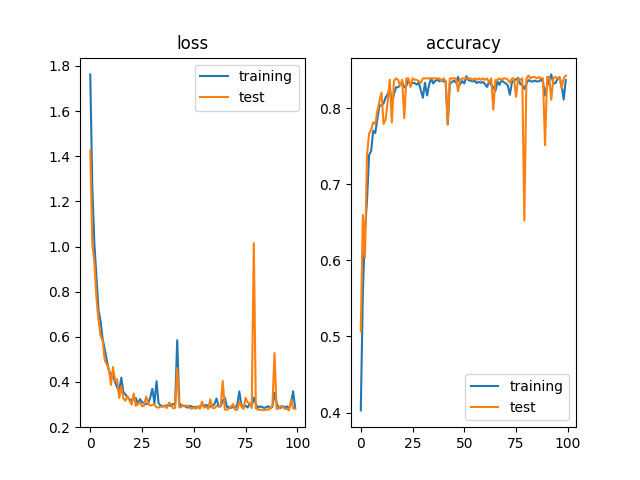
\includegraphics[keepaspectratio, scale=0.3]{images/less_train_fnn.png}
        \subcaption{Simple FNN}
        \label{fig:Simple_FNN}
      \end{minipage}
      \begin{minipage}[b]{0.45\linewidth}
        \centering
        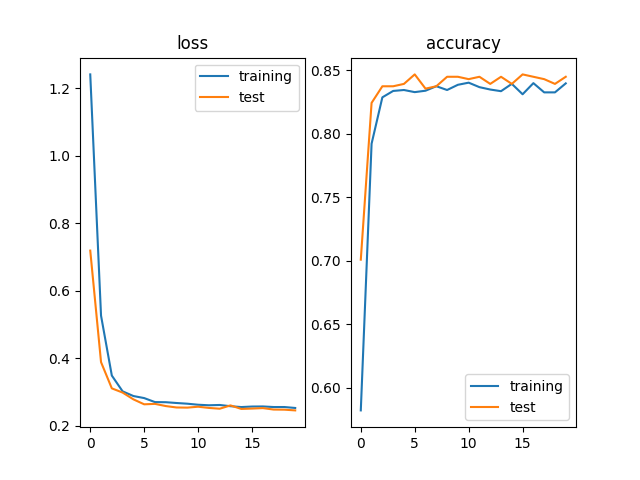
\includegraphics[keepaspectratio, scale=0.3]{images/less_train_cnn.png}
        \subcaption{Simple CNN}
        \label{fig:Simple_CNN}
      \end{minipage}
    \end{figure}    
  \end{frame}

  \begin{frame}{他のデータベースの評価①}
    使用していたデータベース(GPCR)はデータ数が71442であり、ファミリー数は86である。よって、
    単位ファミリーにおける平均データ数は
    \[
      \frac{71442}{86} = 830.72
    \]
    ある。それに対して、より大きなデータベース(COG-100-2892)においてはデータ数が3131952であり、
    ファミリー数は2892である。よって、同様に単位ファミリーにおける平均データ数は
    \[
      \frac{3131952}{2892} = 1082.97
    \]
    となる。単位ファミリーあたりにおけるデータ数はの差は二百程度であるが、データに偏りが大きければ
    あまり意味がない。
  \end{frame}

  \begin{frame}{他のデータベースの評価②}
    他のデータベース(COG-100-2892)について調べた結果を表\ref{fig:bigger_composition}に示す。
    簡単のため、10より小さいファミリーを示した。
    \begin{table}
      \caption{データベースの構成\footnote{sum=3131952, kind=2892}}
      \label{fig:bigger_composition}
      \centering
      \begin{tabular}{llll}
        \hline
        family & count & family & count \\
        \hline \hline
        0 & 1414 & 5 & 3070 \\
        1 & 1256 & 6 & 842 \\
        2 & 880 & 7 & 2483 \\
        3 & 1648 & 8 & 2018 \\
        4 & 1244 & 9 & 1772 \\
        \hline
      \end{tabular}
    \end{table}
    一瞥したが、極端にデータ数が少ないファミリーは少なかった。
  \end{frame}

  \begin{frame}{他のデータベースを用いた学習結果①}
    ニューラルネットワークのモデル(Simple\_FNNとSimple\_CNN)を利用して学習を行い、
    学習結果を表\ref{tab:other_result}に示す。
    \begin{table}
      \caption{学習結果}
      \label{tab:other_result}
      \centering
      \begin{tabular}{ll}
        \hline
        モデル & 精度 \\
        \hline \hline
        Simple\_FNN & 0.42407429218292236 \\
        Simple\_Cov & 1.0 \\
        \hline
      \end{tabular}
    \end{table}
  \end{frame}

  \begin{frame}{削減データを用いた学習結果②}
    また、それぞれのモデルの学習過程を図\ref{fig:other_FNN}と図\ref{fig:other_CNN}にそれぞれ示す。
    \begin{figure}
      \begin{minipage}[b]{0.45\linewidth}
        \centering
        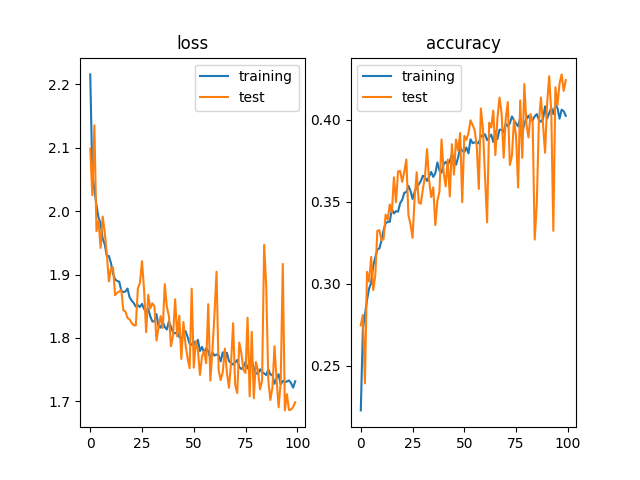
\includegraphics[keepaspectratio, scale=0.3]{images/other_train_fnn.png}
        \subcaption{Simple FNN}
        \label{fig:other_FNN}
      \end{minipage}
      \begin{minipage}[b]{0.45\linewidth}
        \centering
        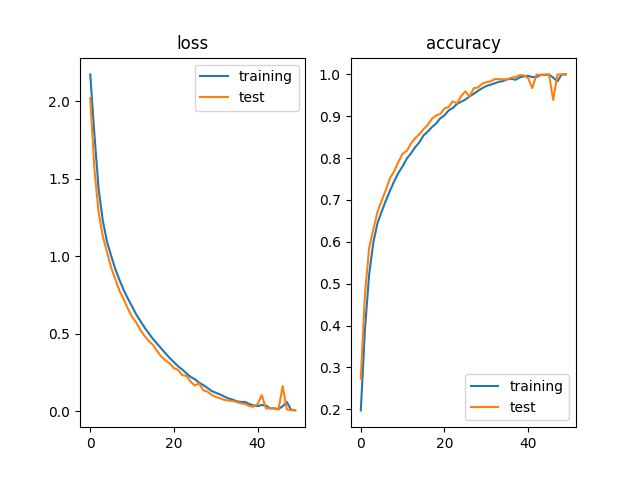
\includegraphics[keepaspectratio, scale=0.3]{images/other_train_cnn.png}
        \subcaption{Simple CNN}
        \label{fig:other_CNN}
      \end{minipage}
    \end{figure}    
  \end{frame}

  \begin{frame}{まとめ}
    \begin{itemize}
      \item データの偏りがあったため、他のデータベースを用いる
      \item それぞれのファミリーのデータ数に偏りをなくす?
      \item 精度が高すぎる原因やテストのほうが精度が高い原因を探る
      \item より複雑なニューラルネットワークモデルを組む
      \item 『ゼロから作るDeep Learning』のニューラルネットワークでモデルを組む
    \end{itemize}
  \end{frame}

\end{document}


